%
% File: chap02.tex
%
\let\textcircled=\pgftextcircled
\chapter{Multigrid}
\label{chap:multigrid}
\initial{T}his chapter introduces some of the basic concepts and equations of multigrid methods. Multigrid methods very often provide higher efficiency than other iterative solvers for various kinds of partial differential equations. Especially for the solution of elliptic partial differential equations they are so useful  that they are generally accepted to be the fastest numerical solver available \cite{Trottenberg:2000:MUL:374106}.

Multigrid algorithms accelerate the rate of convergence of basic iterative methods by correcting the iterative solution with a global error. For that, a residual $d_h^m = f_h - L_h u_h^m$ is defined and an error $v_h^m$ is computed via $L_h v_h^m = d_h^m$. This equation can be solved with the same iteration method as the linear system, but on many different grid levels. In fact, not just the error of the initial approximation is computed, but also the error of this error and errors of other grid levels. 

For this computation, we exploit the fact that the error of iterative methods becomes smooth after very few iterations. When looking at the error on a coarser grid, the formerly smooth error appears to be more rough, and applying the iterative method on this rough grid lessens the error quicker than on a finer grid. Changing back from a coarse to a fine grid yields a quickly converging solution. 

By doing this on multiple levels, the algorithm is much more efficient than regular iterative methods like the Gauss-Seidel or Jacobi method. Solving a system with $n$ unknowns with such an iterative method on its own takes $\mathcal{O}(n^2)$ steps (which is unacceptable for many applications), while multigrid methods only need $\mathcal{O}(n)$ steps. Remarkably, the number of iterations does not increase for bigger grid sizes with multigrid methods. Also, the high extent to which these algorithms can be parallelized makes them suitable for high performance computing. In the following sections, different types of smoothers and the multigrid idea are discussed. 

\section{Basic Ideas of Multigrid}

In this section the basic ideas of multigrid are illustrated. For that, two important observations have to be made.
\subsection{Error Smoothing Through Iterative Methods}
The first observation is that an iterative method produces a smooth error on a grid. Take for example the Gauss-Seidel iteration for the Poisson equation (this equation will be discussed in more detail later):
\begin{align}
\label{equ:gauss-seidel-poisson}
u_h^{m+1}(x_i,y_j) =  \frac{1}{4} [h^2 f_h (x_i, y_j) & +  u_h^{m+1} (x_i-h, y_j) + u_h^{m}(x_i+h, y_j) \nonumber \\ 
& + u_h^{m+1}(x_i, y_j -h) + u_h^{m} (x_i, y_j+h)],
\end{align}
where $(x_i, y_j)$ are points on the grid $\Omega_h$, and $u_h^m$ and $u_h^{m+1}$ are approximations of the exact solution $u_h$ before and after an iteration, respectively. When using (\ref{equ:gauss-seidel-poisson}) to calculate the error 
\begin{equation}
v_h^m(x_i, y_j) = u_h(x_i, y_j) - u_h^m(x_i, y_j),
\end{equation}
it becomes obvious that the iterative formula sets the new error to the average of the four surrounding error values:
\begin{align}
v_h^{m+1}(x_i, y_j) = \frac{1}{4}[&v_h^{m+1}(x_i-h, y_j) + v_h^{m}(x_i+h, y_j)\nonumber \\
 + &v_h^{m+1}(x_i, y_j-h) + v_h^{m}(x_i, y_j + h)].
\end{align}
Of course, averaging the error makes it smooth very quickly, but that does not mean that it becomes small. This effect is illustrated in three figures: Fig.~\ref{fig:mg_error_smoothing_initial} shows the very coarse error of the initial guess. After two iterations, this error became quite smooth, but the absolute value only changed from 1 to around 0.7 (see Fig.~\ref{fig:mg_error_smoothing_2}. After ten iterations of the error smoothing procedure have been applied, the error is very smooth, but still has peaks with a value of 0.6 (Fig.~\ref{fig:mg_error_smoothing_10}). 

\begin{figure}[tbp]
	\centering
	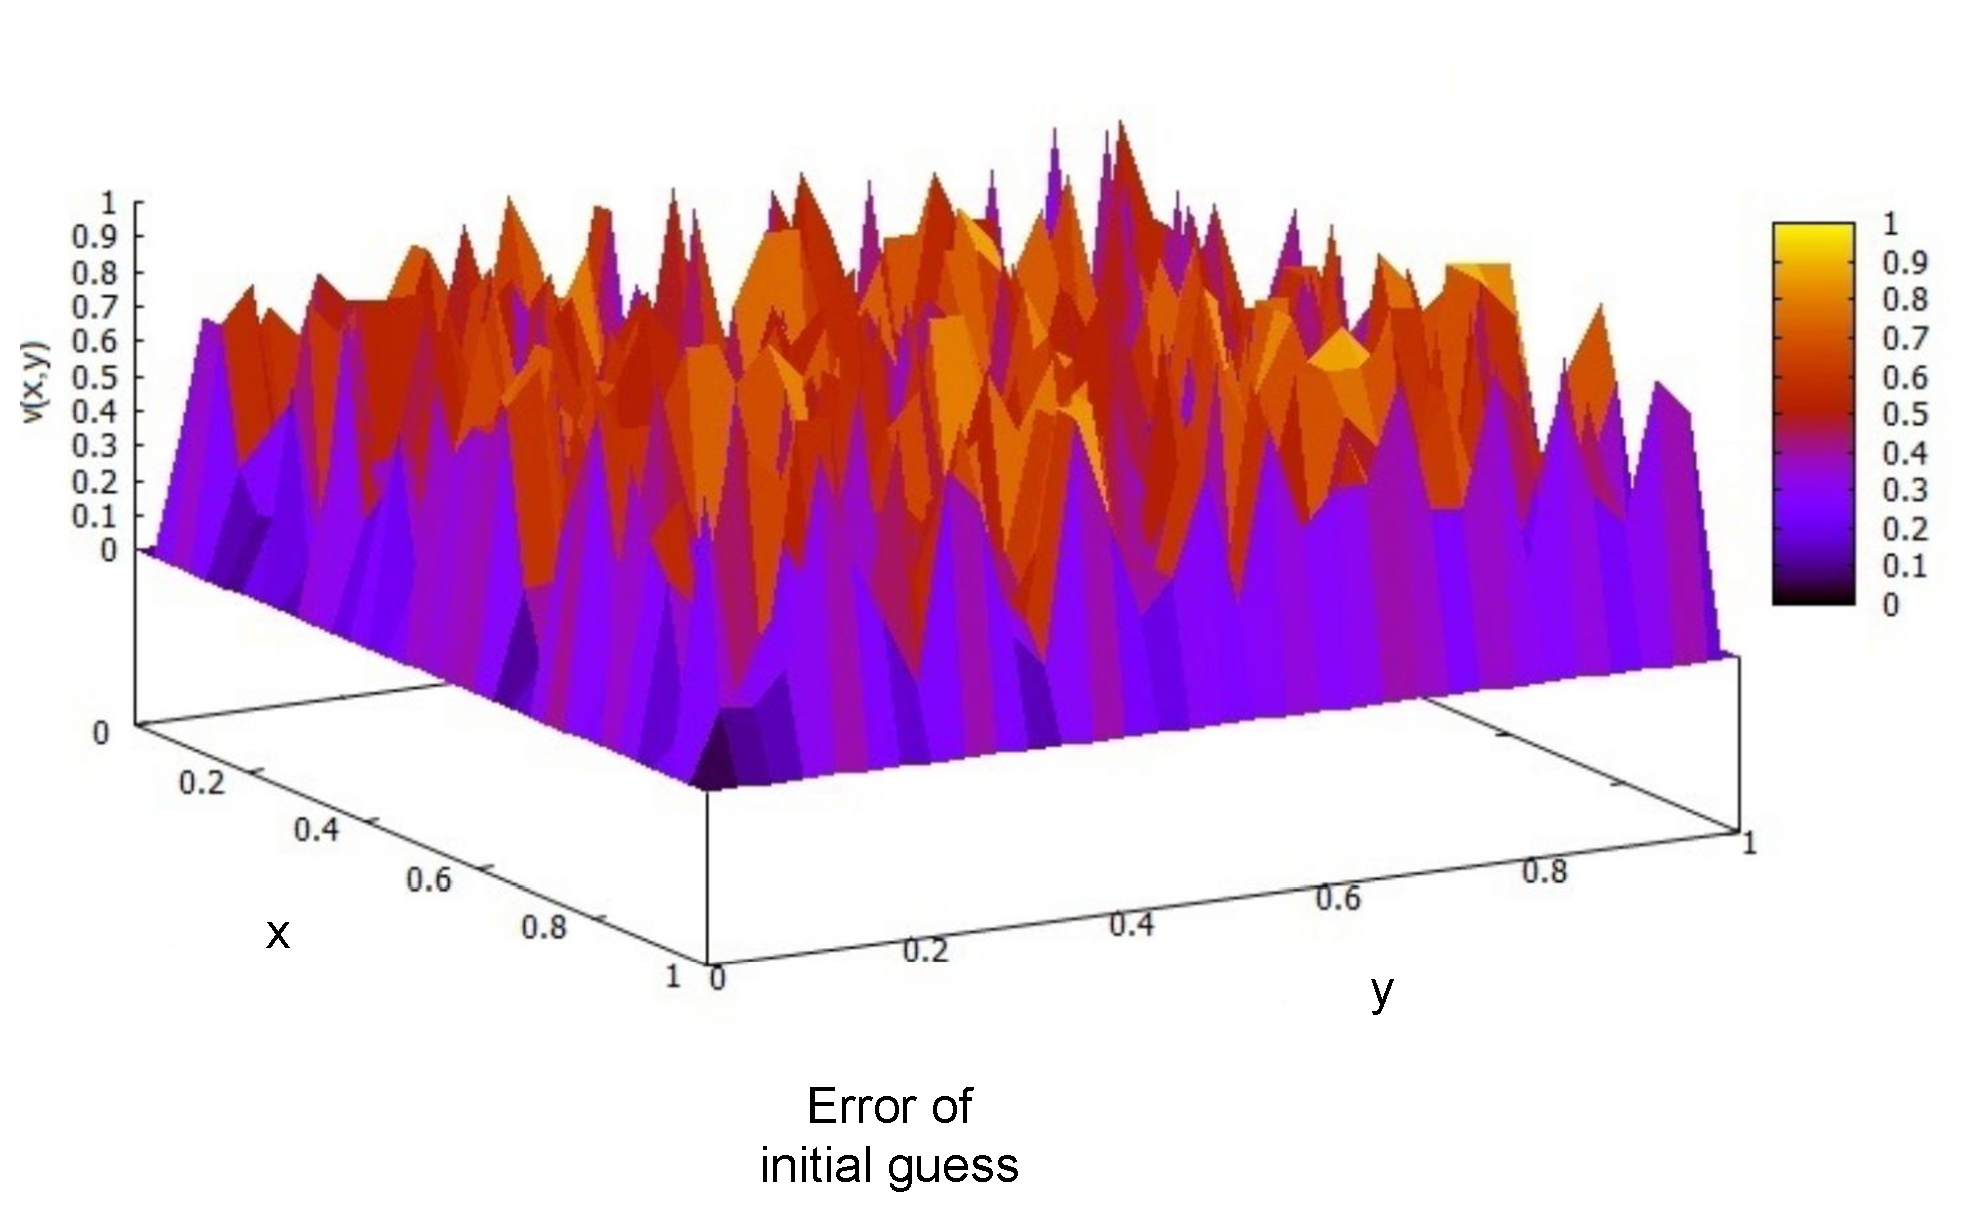
\includegraphics[width=0.9\textwidth]{chapters/chapter02/mg_error_smoothing_initial}
	\caption{The error of an initial guess is very coarse and reaches the highest possible value 1: Later, after smoothing has been applied, it will be much smoother.}
	\label{fig:mg_error_smoothing_initial}
\end{figure}

\begin{figure}[tbp]
	\centering
	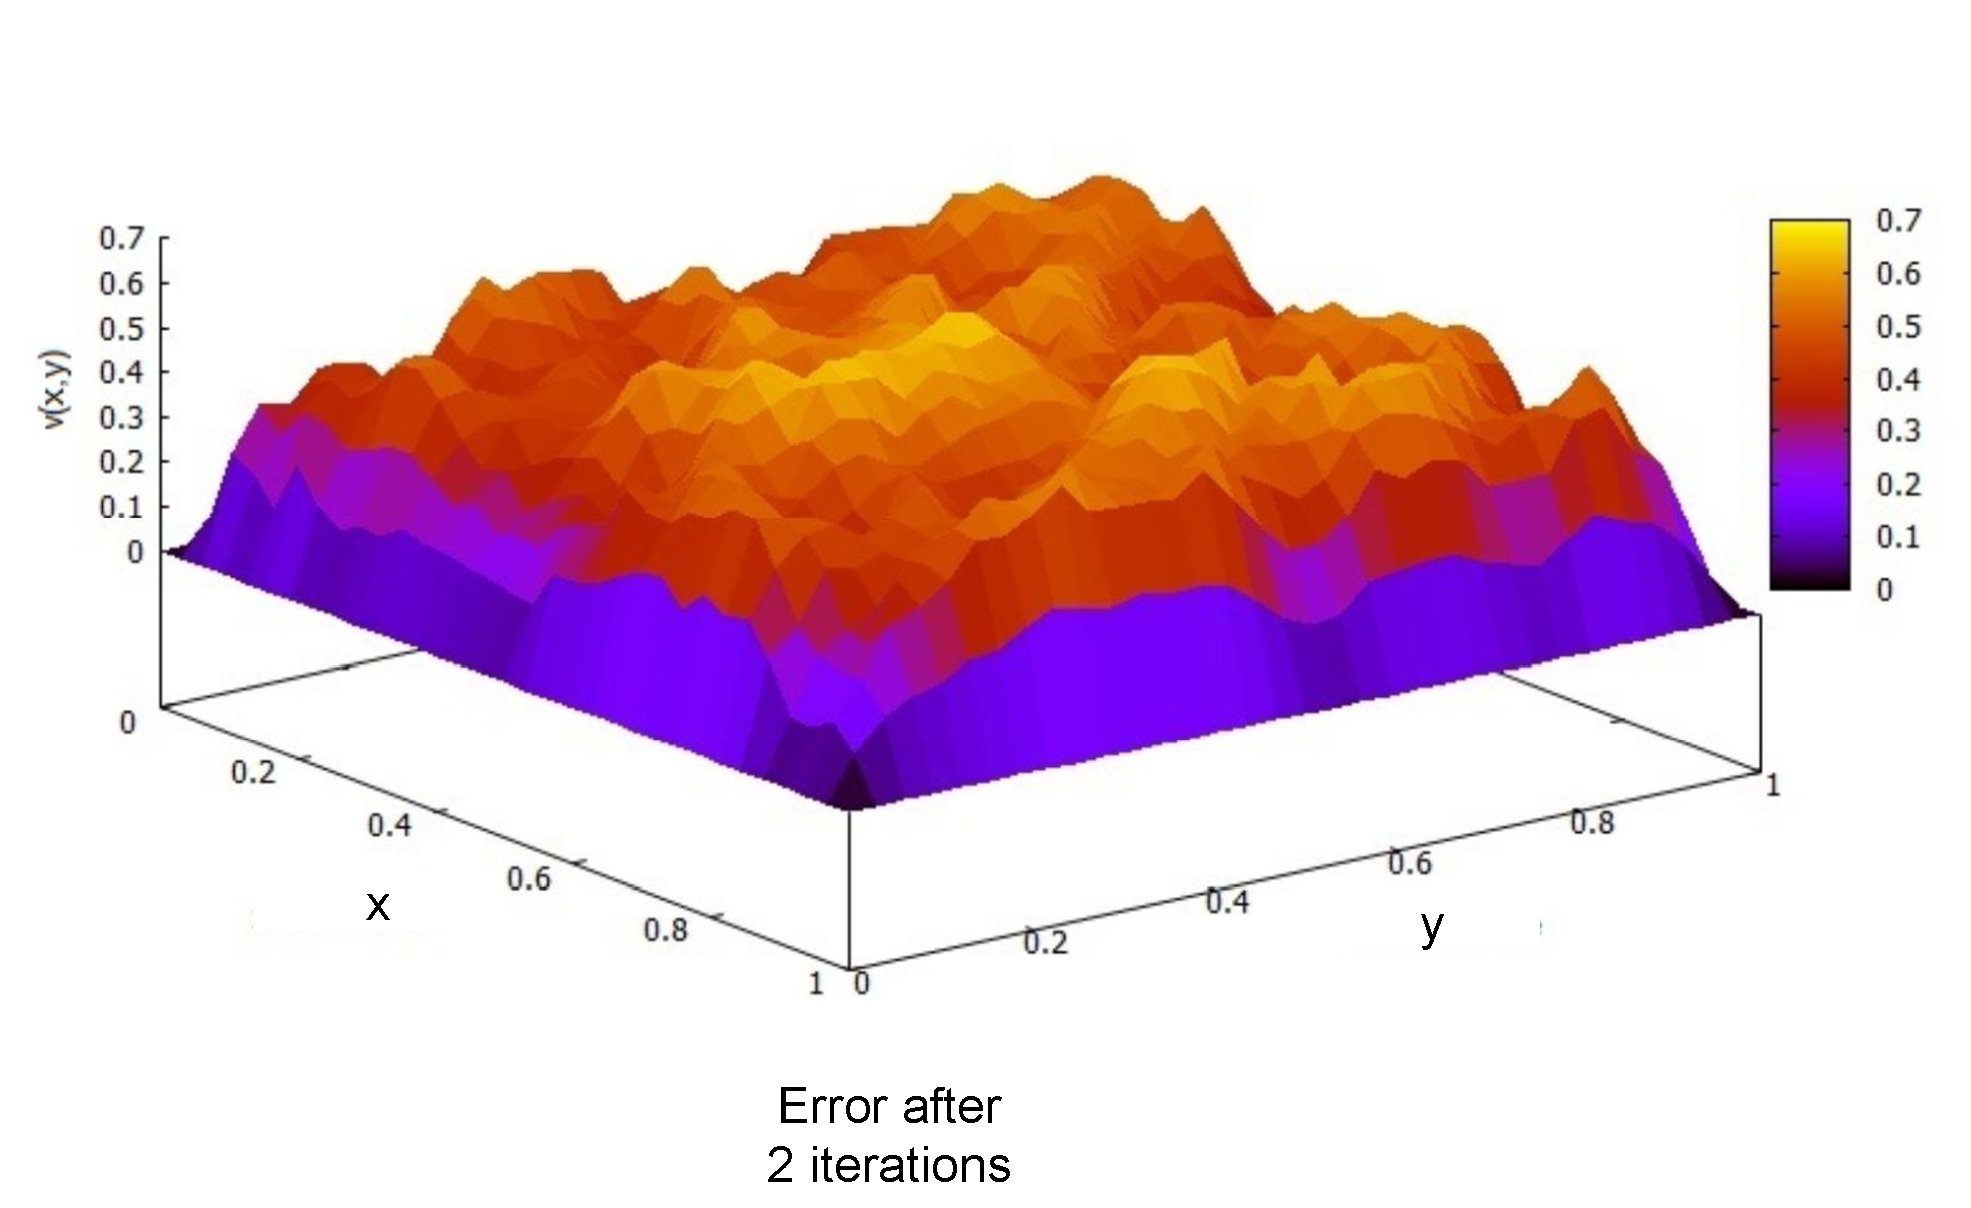
\includegraphics[width=0.9\textwidth]{chapters/chapter02/mg_error_smoothing_2}
	\caption{After only two smoothing iterations, the error is much smoother than after the initial guess. The peaks of the error did not change so much, though: Only a change from 1 to around 0.7 can be observed (compared to Fig.~\ref{fig:mg_error_smoothing_initial}).}
	\label{fig:mg_error_smoothing_2}
\end{figure}

\begin{figure}[tbp]
	\centering
	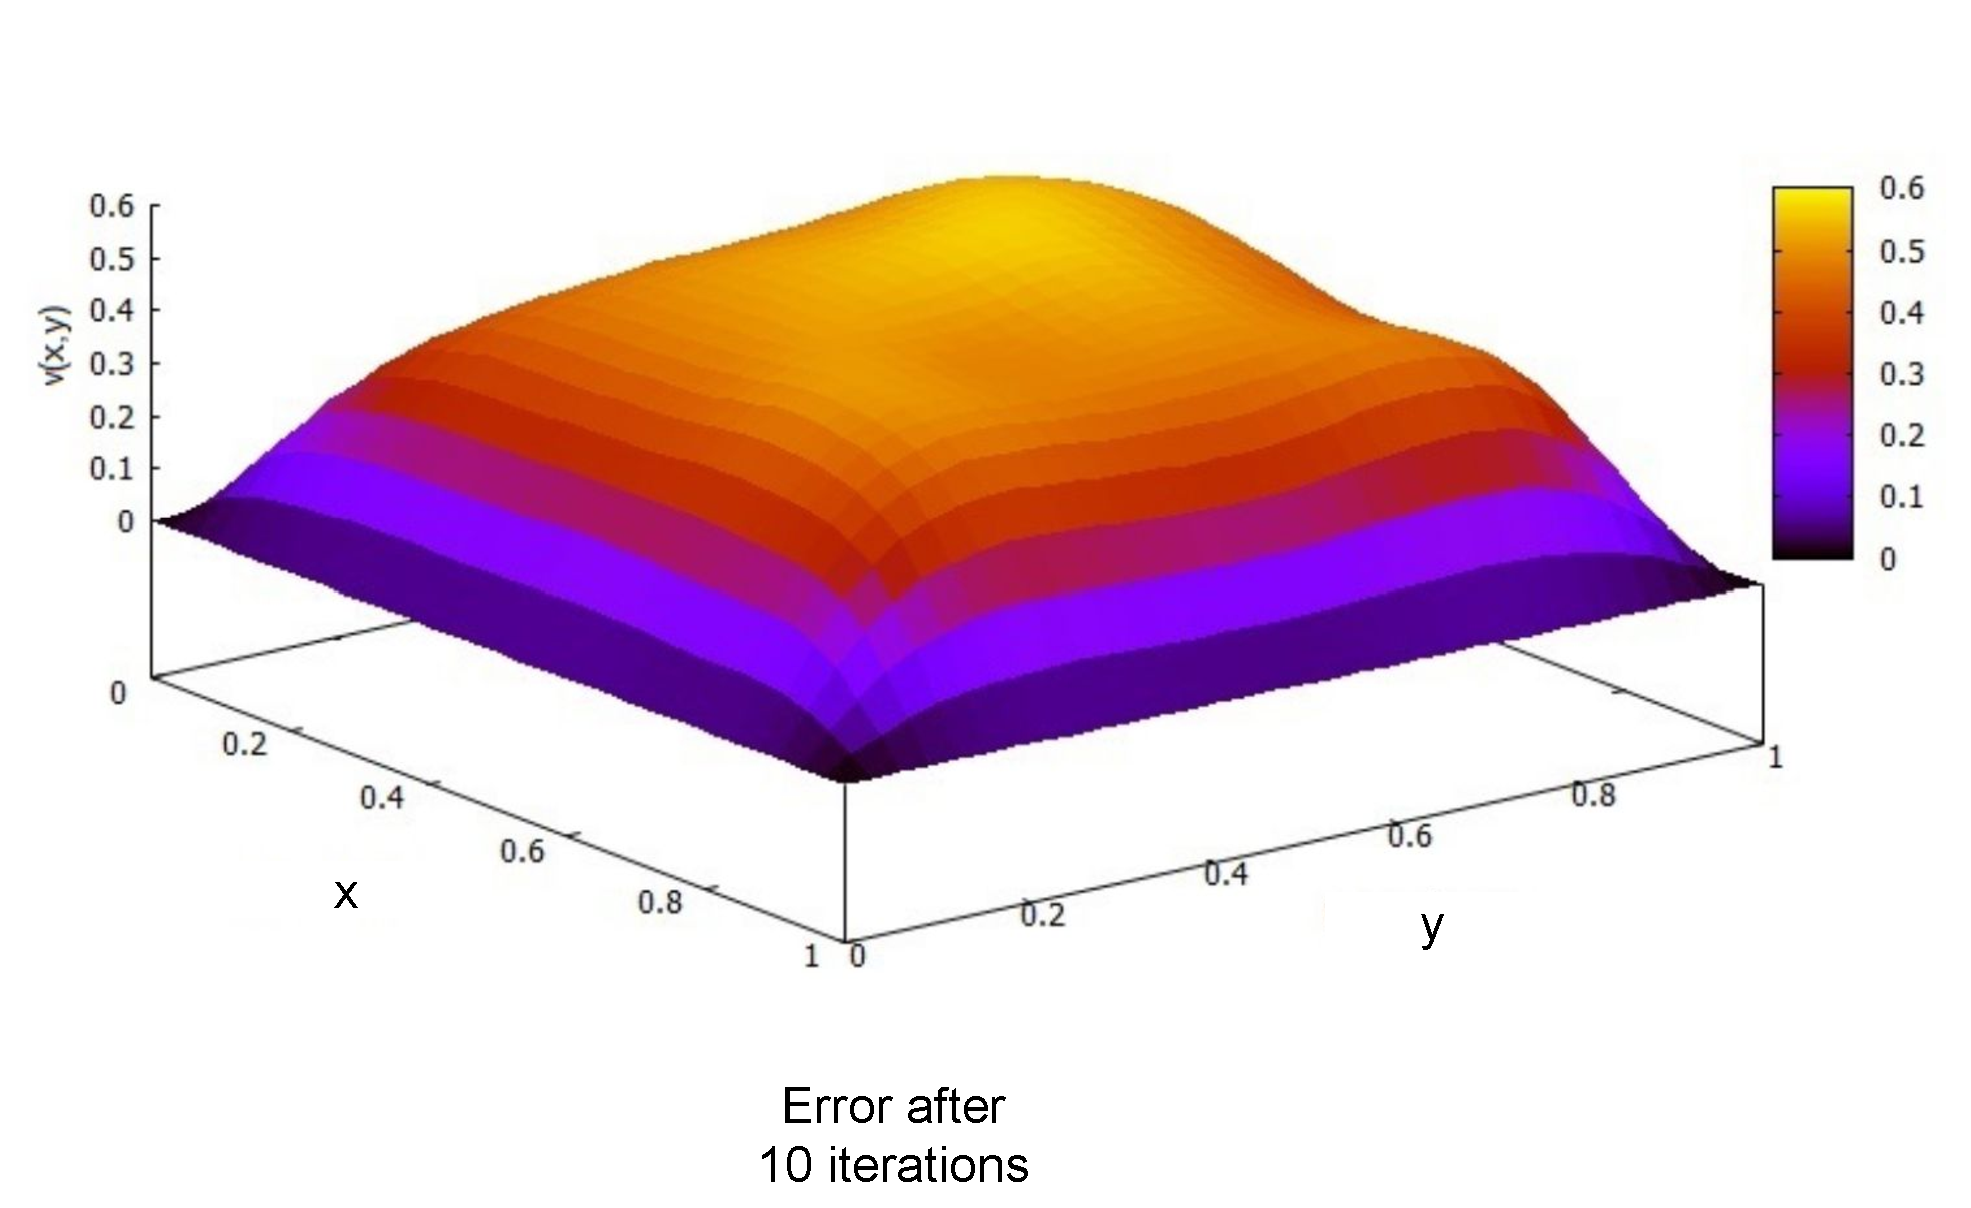
\includegraphics[width=0.9\textwidth]{chapters/chapter02/mg_error_smoothing_10}
	\caption{After 10 iterations the error is very smooth, but the peak of the error only changed from 0.7 after 2 iterations to 0.6 now.}
	\label{fig:mg_error_smoothing_10}
\end{figure}


\subsection{Approximating Smooth Errors on Coarse Grids}
The second observation is that a smooth error on a fine grid can be well approximated on a coarser grid. This is because smoothness implies that there are no distinct high frequency components, which means the solution only needs low frequency components (hence, less information, which can also be provided by fewer grid points) to be approximated well. Therefore, if the error has become smooth after a few iterations, it can be approximated on a much coarser grid, where further computations are less expensive due to fewer grid points.

But what does high and low frequency actually mean? For that, we can express the error with a Fourier expansion as the sum of different sine waves:
\begin{equation}
v_h(x,y) = \sum_{k,l = 1}^{N-1} \alpha_{k,l} \sin k \pi x~ \sin l \pi y.
\end{equation}

We see, this error is a sum of eigenfunctions 
\begin{equation}
\varphi_h ^{k,l}(x,y) = \sin k \pi x~ \sin l \pi y \text{~~~~}(k,l = 1, \hdots, n-1)
\end{equation}
of the discrete operator $L_h$ on the fine grid. Therefore, in that context error smoothing means that low frequency components ($k$ and $l$ are small) are barely changed by smoothing iterations, while high frequency components ($k$ or $l$ is large) become small.

Of course not all frequency components that are visible on a fine grid are also visible on a coarse grid. If the frequency of a component is higher or equal to half the number of grid points $N$, this component appears to have a lower frequency. 
This effect is called aliasing and means that the eigenfunctions of a fine grid $\Omega_h$
\begin{equation*}
\varphi^{k,l}, \text{~~~~~~~~~}\varphi^{N-k,N-l}, \text{~~~~~~~~~}\varphi^{N-k,l}, \text{~~~~~~~~~}\varphi^{k,N-l}, 
\end{equation*}
all appear to have the same frequency on a grid with twice the mesh size $\Omega_{2h}$:
\begin{equation}
\varphi^{k,l}(x,y) = - \varphi^{N-k,l}(x,y) = -\varphi^{-k,N-l}(x,y) = \varphi^{n-k,N-l}(x,y)  \text{~~~for~~}  (x,y) \in \Omega_{2h} 
\end{equation}


\begin{figure}[h]
	\centering
	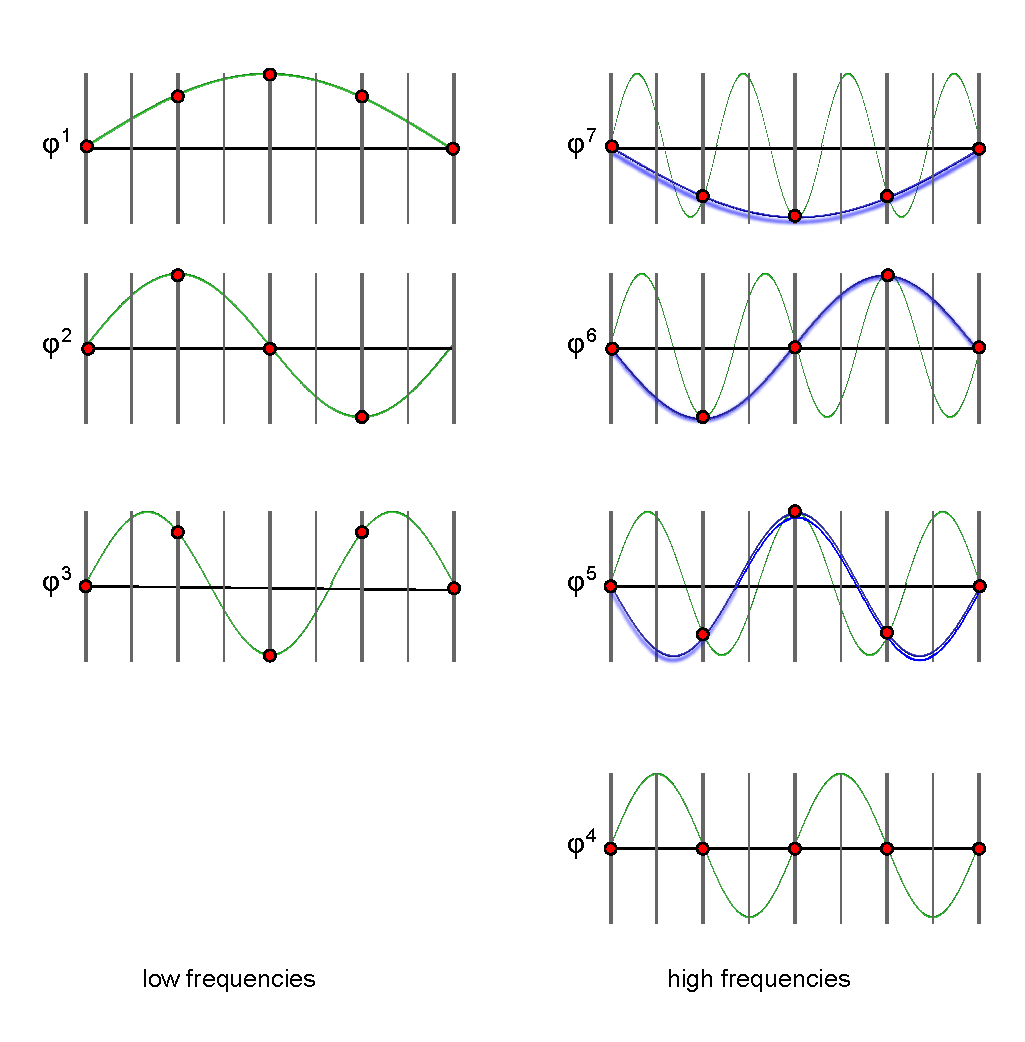
\includegraphics[width=1.\textwidth]{chapters/chapter02/mg_low_aliasing}
	\caption{All vertical lines correspond to a 1D fine grid with $N = 8$, while only the thick lines belong to a coarse grid. Only the eigenfunctions with low frequencies $\varphi^1 - \varphi^3$ appear correctly on the coarse grid, while $\varphi^4$ is not visible at all and $\varphi^5 - \varphi^7$ appear as an inverted eigenfunction of lower frequency, drawn with a thick blue line ($\varphi^5$ seems to be $-\varphi^3$, etc.).}
	\label{fig:mg_aliasing}
\end{figure}


For the case that one of the two frequencies of the eigenfunction is the same as the frequency of the coarse grid, this eigenfunction completely vanishes on $\Omega_{2h}$:
\begin{equation}
\varphi^{N/2,~l}(x,y) = \varphi^{k,~N/2}(x,y) = 0  \text{~~~for~~}  (x,y) \in \Omega_{2h} 
\end{equation}
These aliasing effects are illustrated in Fig.~\ref{fig:mg_aliasing}, which shows an example of a one-dimensional grid with $N = 8$:  The eigenfunctions $\varphi^5-\varphi^7$ appear on the coarse grid like the inverted version of the corresponding eigenfunction with low frequency, while $\varphi^4$ is not visible at all on the coarse grid.
Therefore, eigenfunctions with frequencies $k, l < N~/~2$ are said to have a low frequency, and all other eigenfunctions (which do not appear correctly on the coarse grid) are said to have high frequencies.





\section{Iterative Methods as Smoothers}
As it has been sketched in the beginning of this chapter, iterative solvers are capable of smoothing the error $v_h^m$ of an approximation $u_h^m$ considerably. Which solver (smoother) is selected and the choice of its relaxation parameter $\omega$ have a crucial impact on the smoothing properties. However, good smoothing properties might interfere with the degree of parallelization, since this degree also depends on the ordering of grid points.

The Jacobi and the Gauss-Seidel iterations have already been described in the first chapter as a means of solving a linear system. As it is very important to obtain a smooth error (and not primarily to get a small error), the particularly good error smoothing capabilities of these iterations are utilized to that end. When these iterations are used as smoothers, they are often called relaxation methods rather than iterative solvers. 


\subsection{Jacobi Relaxation}
The ordering of grid points was assumed to already be selected when iterative methods were introduced in Chapter 1, so $u_h^m$ and $f_h^m$ were one dimensional vectors. Here however, we use the explicit two-dimensional indication of a point's position on the grid again. Then the Jacobi relaxation reads 
\begin{align}
z_h^{m+1}(x_i, y_i)&= \frac{1}{4} \Big ( h^2 f_h(x_i, y_i) + u_h^m(x_i-h, y_j) + u_h^m(x_i+h, y_j) \nonumber \\
                  &~~~~~~~~~~~~~~~~~~~~~~~~~~+ u_h^m(x_i, y_j-h) + u_h^m(x_i,y_j+h) \Big ) \\
                  &= \frac{h^2}{4} f_h + \frac{1}{4} \begin{bmatrix}
                  &1 \\
                  1 & & 1\\
                  & 1& 
                  \end{bmatrix}_h u_h^m \nonumber \\
                  & = \frac{h^2}{4} f_h + S_h u_h^m \nonumber \\
        u_h^{m+1} &= z_h^{m+1} & \nonumber
\end{align}
 with the old approximation $u_h^{m}$, the new approximation $u_h^{m+1}$ and with an iteration operator 
 \begin{equation}
 S_h = I_h - \frac{h^2}{4} L_h,
 \end{equation}
 where $I_h$ is the identity operator and $L_h$ is the discretized version of an linear operator $L$. The computation of the mean of the four grid points adjacent to $u_h(x_i, y_j)$ already indicates some kind of smoothing, which will be analyzed shortly. 
 
The Jacobi relaxation can be generalized to the $\omega$-Jacobi relaxation
\begin{equation}
u_h^{m+1} = u_h^m + \omega (z_h^{m+1}-u_h^m),
\end{equation}
where the special case of $\omega = 1$ is the regular Jacobi relaxation. Then the iteration operator for $\omega$-JAC is 
\begin{equation}
S_h(\omega) = \frac{\omega}{4} \begin{bmatrix}
                  &1 \\
                  1 & 4(1/\omega -1) & 1\\
                  & 1& 
                  \end{bmatrix}_h\\
\end{equation}

The value of the relaxation parameter $\omega$ influences the smoothing properties of the relaxation method. In order to analyze this effect, we look at the eigenfunctions and eigenvalues of $S_h$. Since $S_h$ is a linear combination of $L_h$ and $I_h$, the eigenfunctions are the same as the ones of $L_h$:
\begin{equation}
\varphi_h ^{k,l}(x,y) = \sin k \pi x~ \sin l \pi y \text{~~~~}(k,l = 1, \hdots, n-1)
\end{equation}
with corresponding eigenvalues 
\begin{equation}
\chi_h^{k,l}(\omega) = 1- \frac{\omega}{2}(2-\cos k \pi h - \cos l \pi h)
\label{equ:eigenvalues}
\end{equation}

The smoothing factor of the $\omega-$JAC relaxation is the factor by which high-frequency components of the error are reduced per iteration step in the worst case. It is defined as the greatest absolute value of the eigenvalues of the high frequency eigenfunctions:
\begin{equation}
\mu (h,\omega) = \max \Big\{\Big|\chi_h^{k,l}(\omega)~\Big|: n~/~2 ~\leq ~\max(k,l) ~\leq ~n-1 \Big\} 
\end{equation}
The supremum $\mu^*$ over $h$  gives the worst case smoothing factor over all grids. Here, it is reasonable to set $h$ of the coarsest grid on which smoothing is applied to $h = 1/4$~\cite{Trottenberg:2000:MUL:374106}. Inserting the eigenvalues of (\ref{equ:eigenvalues}) into the equation for the smoothing factor yields a supremum 
\begin{equation}
\mu^* (\omega) = \max \big\{\big|1-\omega/2\big|,~\big|1-2\omega\big| \big\}.
\end{equation}


The case for $\omega = 4/5$ is particularly important because it yields the optimal smoothing factor for the $\omega$-Jacobi relaxation:
\begin{equation}
\mu^*(4/5) = 3/5.
\end{equation}
This means every smoothing step with $\omega = 4/5$ reduces high frequencies by at least a factor of 3/5.

\subsection{Gauss-Seidel Relaxation}
The Gauss-Seidel relaxation is again very similar to the Jacobi relaxation, and only differs in the fact that it uses updated function values whenever possible. Again, we use a generalization with a relaxation parameter $\omega$:
\begin{align}
z_h^{m+1}(x_i, y_i)&= \frac{1}{4} \Big ( h^2 f_h(x_i, y_i) + u_h^{m+1}(x_i-h, y_j) + u_h^m(x_i+h, y_j) \nonumber \\
                  &~~~~~~~~~~~~~~~~~~~~~~~~~~+ u_h^{m+1}(x_i, y_j-h) + u_h^m(x_i,y_j+h) \Big ) \\
        u_h^{m+1} &= u_h^m \omega (z_h^{m+1} - u_h^m) & \nonumber
\end{align}
This iteration has much better smoothing properties than the Jacobi iteration. However, these properties now depend on the ordering of grid points. That is because the selection of the grid points that are to be updated first and subsequently used for the calculation of new grid points depends on the ordering: For the red-black ordering, half of the grid points are determined with grid points values that were calculated in the previous iteration and the other half uses "fresh" values from the same iteration. For the lexicographical ordering, the calculation of new grid points needs two new and two old approximations for each point. This choice of ordering also affects the degree of parallelism, as will be shown shortly. 

For the Gauss-Seidel iterations, no detailed analysis of the smoothing properties is given here, but the results are as follows: For lexicographical ordering the optimal smoothing factor is $\mu = 0.5$  and  for red-black ordering it is $\mu = 0.25$, both are obtained with $\omega = 1$. 


\subsection{Comparison: Jacobi and Gauss-Seidel Smoothers}

For high performance computing, the parallel properties of relaxation methods are especially important. For example, the $\omega$-Jacobi method does not have any sequential dependencies, that means all new approximations of grid point values can be computed at the same time. The degree of parallelism is therefore the same as the number of grid points in $\Omega_h$:
\begin{equation}
\text{par-deg}(\omega\textrm{-JAC}) = \#\Omega_h
\end{equation}

On the other hand, the degree of parallelism for the Gauss-Seidel relaxation depends on the ordering: For lexicographical order, a grid point can only be computed if the updated values of two adjacent grid points, that are not opposite to each other, are already updated, as shown in Fig.~\ref{fig:mg_parallel_properties}a). Hence, the grid points have to be calculated one diagonal after another, as illustrated in Fig.~\ref{fig:mg_parallel_properties}b). The degree of parallelism is then
\begin{equation}
\text{par-deg}(\textrm{GS-LEX}) \leq \sqrt{\#\Omega_h}
\end{equation}

If the numbering of grid points follows a red-black order (see Fig.~\ref{fig:mg_parallel_properties}c)), the situation is completely different: Now the Gauss-Seidel iteration can be applied to all black grid points simultaneously and after that, it is applied to the red grid points by using the just updated values of black grid points. Since half of the grid points can be processed at the same time, the degree of parallelism is 
\begin{equation}
\text{par-deg}(\textrm{GS-RB}) = \frac{1}{2} \#\Omega_h.
\end{equation}



\begin{figure}[h]
	\centering
	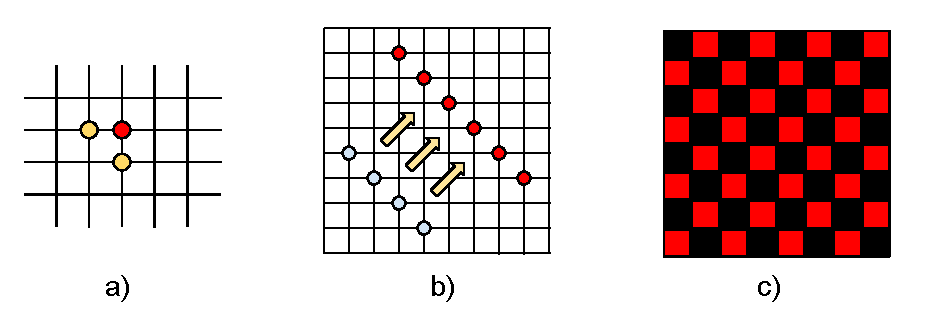
\includegraphics[width=1.\textwidth]{chapters/chapter02/mg_parallel_properties}
	\caption{\textbf{a)} In order to calculate the value of the red point with the lexicographical Gauss-Seidel iteration, the yellow points already have to be updated. \textbf{b)} Because of a), one diagonal is processed after another with the lexicographical Gauss-Seidel method. \textbf{c)}~With the Gauss-Seidel iteration using red-black ordering, first all black points can be processed at the same time, then the iteration is applied to the red points by using the updated black point values.}
	\label{fig:mg_parallel_properties}
\end{figure}

\begin{table}[]
\centering
\caption{Smoothing properties of different relaxation schemes.}
\label{table:smoothing}
\begin{tabular}{lccc}
\hline
\multicolumn{1}{l}{Relaxation} & \multicolumn{1}{l}{Smoothing factor} & Smoothing & \multicolumn{1}{l}{Parallel degree} \\ \hline
$\omega$-JAC, $\omega = 1$     & 1                                    & No                            & \#$\Omega_h$                        \\
$\omega$-JAC, $\omega = 0.5$   & 0.75                                 & Unsatisfactory                & \#$\Omega_h$                        \\
$\omega$-JAC, $\omega = 0.8$   & 0.6                                  & Acceptable                    & \#$\Omega_h$                        \\
GS-LEX, $\omega = 1$           & 0.5                                  & Good                          & $\leq \sqrt{\#\Omega_h}$        \\
GS-RB, $\omega = 1$            & 0.25                                 & Very good                     & $\frac{1}{2}\#\Omega_h$                         
\end{tabular}
\end{table}

These results are summarized in Table.~\ref{table:smoothing}. So the $\omega-$Jacobi relaxation is fully parallel, but its smoothing properties are just moderate, in the best case. For $\omega = 1$, high frequency components are not smoothed at all in the worst case. Gauss-Seidel relaxation on the other hand has excellent smoothing properties for the red-black ordering and a high parallel degree of $\frac{1}{2}\Omega_h$. It should be noted though that this smoothing factor is only valid if at most two smoothing steps are performed \cite{Trottenberg:2000:MUL:374106}. 


\subsection{Other Smoothing Methods}
There are many other methods to solve a linear system $Au = f$, but only some of them are suitable as smoothers. Direct solvers, like the Gaussian elimination or LU decomposition are a bad choice, because they are wasteful and very time consuming for the solution of large systems \cite{mazumder2015numerical}. This is partly due to the fact that a direct solver always has to solve the system from the start, while iterative solvers can start from approximations that may already be close to the solution~\cite{ascher2011first}.

Such an iterative solver can basically be any iteration that smooths the error, among them are the line-by-line method \cite{mazumder2015numerical},  Stone's Strongly Implicit Method \cite{stone1968iterative}, the Method of Steepest Descent \cite{mazumder2015numerical}, the Modified Richardson iteration \cite{richardson1911ix} or the Conjugate Gradient method \cite{hestenes1952methods}. However, the Jacobi and the Gauss-Seidel method proved to be the most suitable ones \cite{Trottenberg:2000:MUL:374106}.



\section{Two-Grid Cycle}
As mentioned before, the two main principles of two-grid and multigrid cycles are the error smoothing properties of relaxation methods and the fact that smooth errors can be well approximated on coarse grids. Now the steps in which these two principles are performed will be discussed, starting with the two-grid cycle. For that, we define the error of the solution as the vector difference between the exact solution $u_h$ and the approximation $u_h^m$:
\begin{equation}
v_h^m \coloneqq u_h - u_h^m.
\end{equation}
The defect (also called residual) is then
\begin{equation}
d_h^m \coloneqq f_h - L_h u_h^m
\end{equation}
and the defect equation is 
\begin{equation}
L_h v_h^m = d_h^m.
\label{eq:mg_defect}
\end{equation}
Since this equation has the same form as the original problem $L_hu_h^m = f_h$, the same iterative solver can be used. In order to make use of the coarse grid correction, (\ref{eq:mg_defect}) will be used on the coarser grid with $H = 2h$:
\begin{equation}
L_H v_H^m = d_H^m.
\end{equation}

We see why it is much cheaper to solve the system on the coarse grid, when we take a look at the sizes of the corresponding system matrices again: Since the system has $N^2$ unknowns, the number of grid points (unknowns) quarters when increasing the grid size from $h$ to $2h$.

Now we define an algorithm for the two-grid cycle. One such a cycle is a single iteration, so each cycle updates the solution vector. This cycle can be described as a function that takes the following input: 
\begin{itemize}
\item an approximation of the unknown $u_h^{m}$,
\item a linear operator $L_h$ (which is an approximation of $L$),
\item the function $f_h$, and
\item the numbers of presmoothing and postsmoothing steps, \(\nu_1 \textrm{ and }  \nu_2\) 
\end{itemize}
The output is a new approximation $u_h^{m+1}$. The basic steps in this algorithm are presmoothing, the coarse grid correction, and postsmoothing, as shown in Algorithm~1.

\begin{algorithm}
\fbox{%
\begin{minipage}{0.94\textwidth}
\textbf{Two-Grid Cycle:} \hspace{20mm} $u_h^{m+1} = \textbf{twoGridCycle}(u_h^m, L_h, f_h, \nu_1, \nu_2)$
\begin{enumerate}
\item \textbf{Presmoothing:} A relaxation method (e.g. Gauss-Seidel or Jacobi) has be be applied to smooth $u_h^m$ and obtain a smooth $\overline{u}_h^m$.
\item \textbf{Coarse grid correction:} 
\begin{enumerate}
\item Compute the defect on the fine grid: $\hspace{10mm}\quad \quad \quad \quad \overline{d}_h^m = f_h - L_h \overline{u}_h^m$
\item Transfer the defect to the coarse grid:  $\hspace{10mm}\quad \quad \quad \overline{d}_H^m = I_h^H \overline{d}_h^m$
\item Compute the exact error $v_H^m$ on the coarse grid: $ ~~\quad L_H v_H^m = \overline{d}_H^m$
\item Transfer the error to the fine grid: $\hspace{10mm}~~\quad \quad  \quad \quad v_h^m = I_H^h v_H^m$
\item Compute a new approximation: $\hspace{10mm}\quad \quad \quad \quad \quad \quad   u_h^{new} = \overline{u}_h^m + v_h^m$
\end{enumerate}
\item \textbf{Postsmoothing:} The new approximation $u_h^{m+1}$ is obtained through smoothing $u_h^{new}.$
\end{enumerate}
\vspace{1mm}
\end{minipage}}
\vspace{5mm}
\label{alg:two_grid_cycle}
\caption{Two-grid cycle}
\end{algorithm}

Performing the coarse grid correction on its own would not do any good, since the solution would not converge, so smoothing is an essential part of this process. 


%%end of this section
The iteration with a two grid cycle shows much better convergence properties than the iterative solvers working on their own, however, there is still much room for improvement. The error computation in Step 2c) does not converge quickly, so this step can be computed on a coarser grid, where a solution converges faster. The goal is to perform the calculation $Av = r$ on a grid of a particular size, e.g. with $h = 1/4$, independent of the number of grid points $N$. To that end, several grids are used, a procedure that will be discussed in Section~\ref{sec:multigrid_cycle}. Now, we take a closer look at the different steps of the components of the two grid and multigrid procedures.%cite alex


\section{Multigrid Components}
In the two-grid cycle that has just been described, there are three major steps: presmoothing, coarse grid correction and postsmoothing. The smoothing procedures have already been discussed, but some of the components of the coarse grid correction need further explanation. 

\subsection{Restriction}
Step 2b) of the two-grid cycle is transferring the defect to a fine grid. Such a transition from one grid to another can be done in various ways. For our applications, transitions (either from coarse to fine or vice versa) always change the distance between two adjacent points by a factor of two. For the restriction, where only every other point of the fine grid is used, this means the grid changes from a $\Omega_{h}$ to a $\Omega_{2h} = \Omega_H$ grid, so the total number of grid points is quartered. Fig.~\ref{fig:mg_restriction} shows such a restriction. 

\begin{figure}[h]
	\centering
	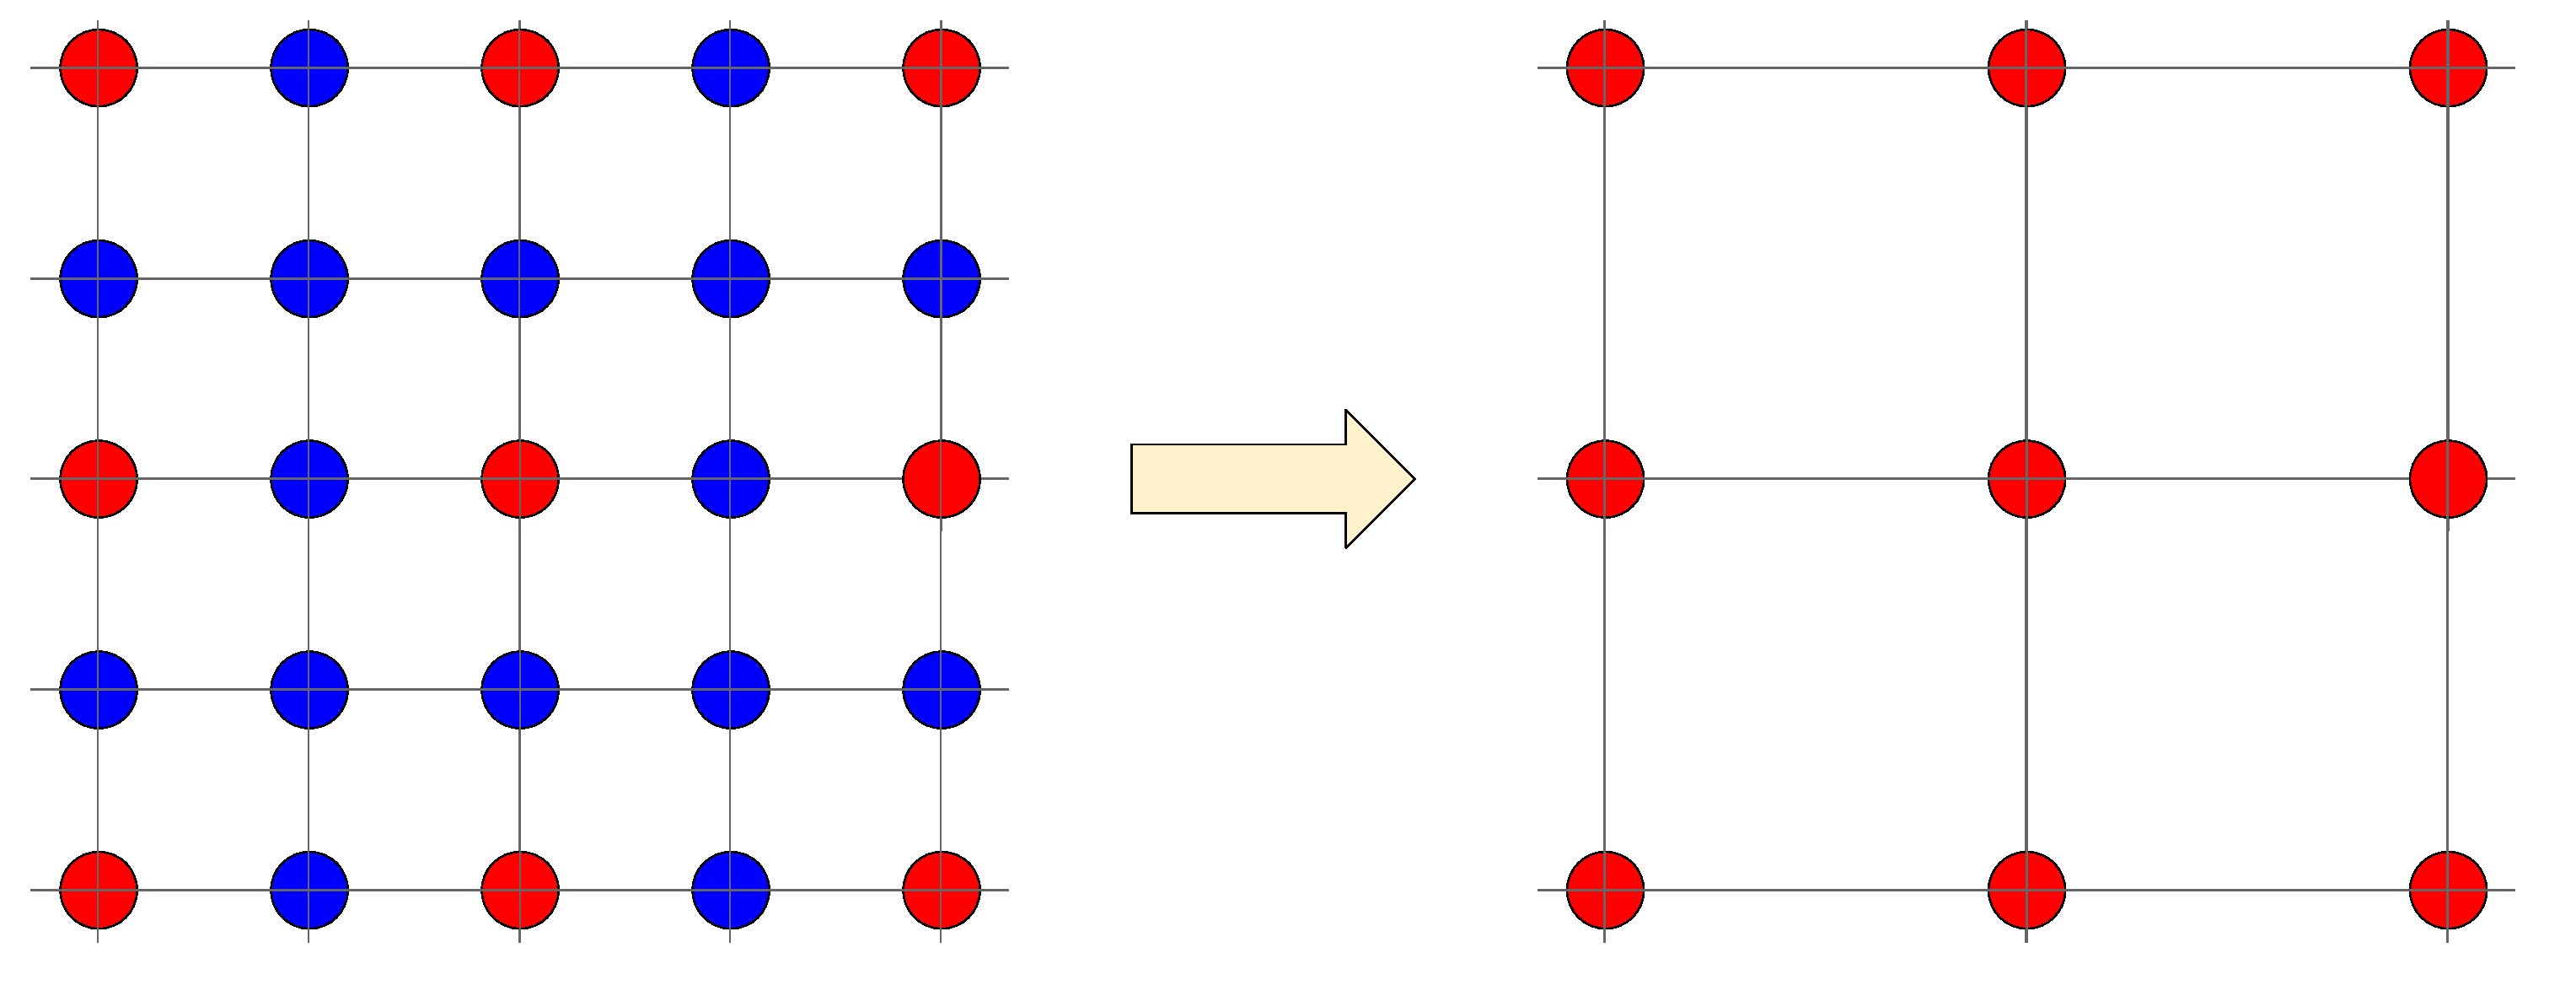
\includegraphics[width=0.7\textwidth]{chapters/chapter02/mg_restriktion}
	\caption{When transferring from a grid $\Omega_h$ to $\Omega_H$, the distance between adjacent grid points doubles from $h$ to $H$.}
	\label{fig:mg_restriction}
\end{figure}

In order to describe a restriction of any grid function $d_h$ to $d_H$, we write
\begin{equation}
d_H(P) = I_h^H d_h(P)~~~~~~~~ \textrm{for } P \in \Omega_H \subset \Omega_h,
\end{equation}
with a restriction operator $I_h^H$. There are different ways to move from $\Omega_h$ to $\Omega_H$, i.e. different ways to define $I_h^H$. The simplest way is to just use the corresponding fine grid points for the coarse grid points, a method called \textbf{injection}.  With the injection operator the restriction can be written as 
\begin{align}
d_{2h}(x,y) &= I_h^{2h} d_h(x,y)\nonumber \\
&=\begin{bmatrix}
\\
& 1 &\\
\\
\end{bmatrix}_h^{2h} d_h(x,y) \\
& = d_h(x,y) \nonumber
\end{align}
So for each point on $\Omega_H$, three points of $\Omega_h$ are completely discarded without using them in any way. Clearly, there are ways to perform a more elegant (i.e. a smoother) transition. For example, there are the full weighting and the half weighting operator, where nine-point and five-point averages are calculated. 


\begin{figure}[h]
	\centering
	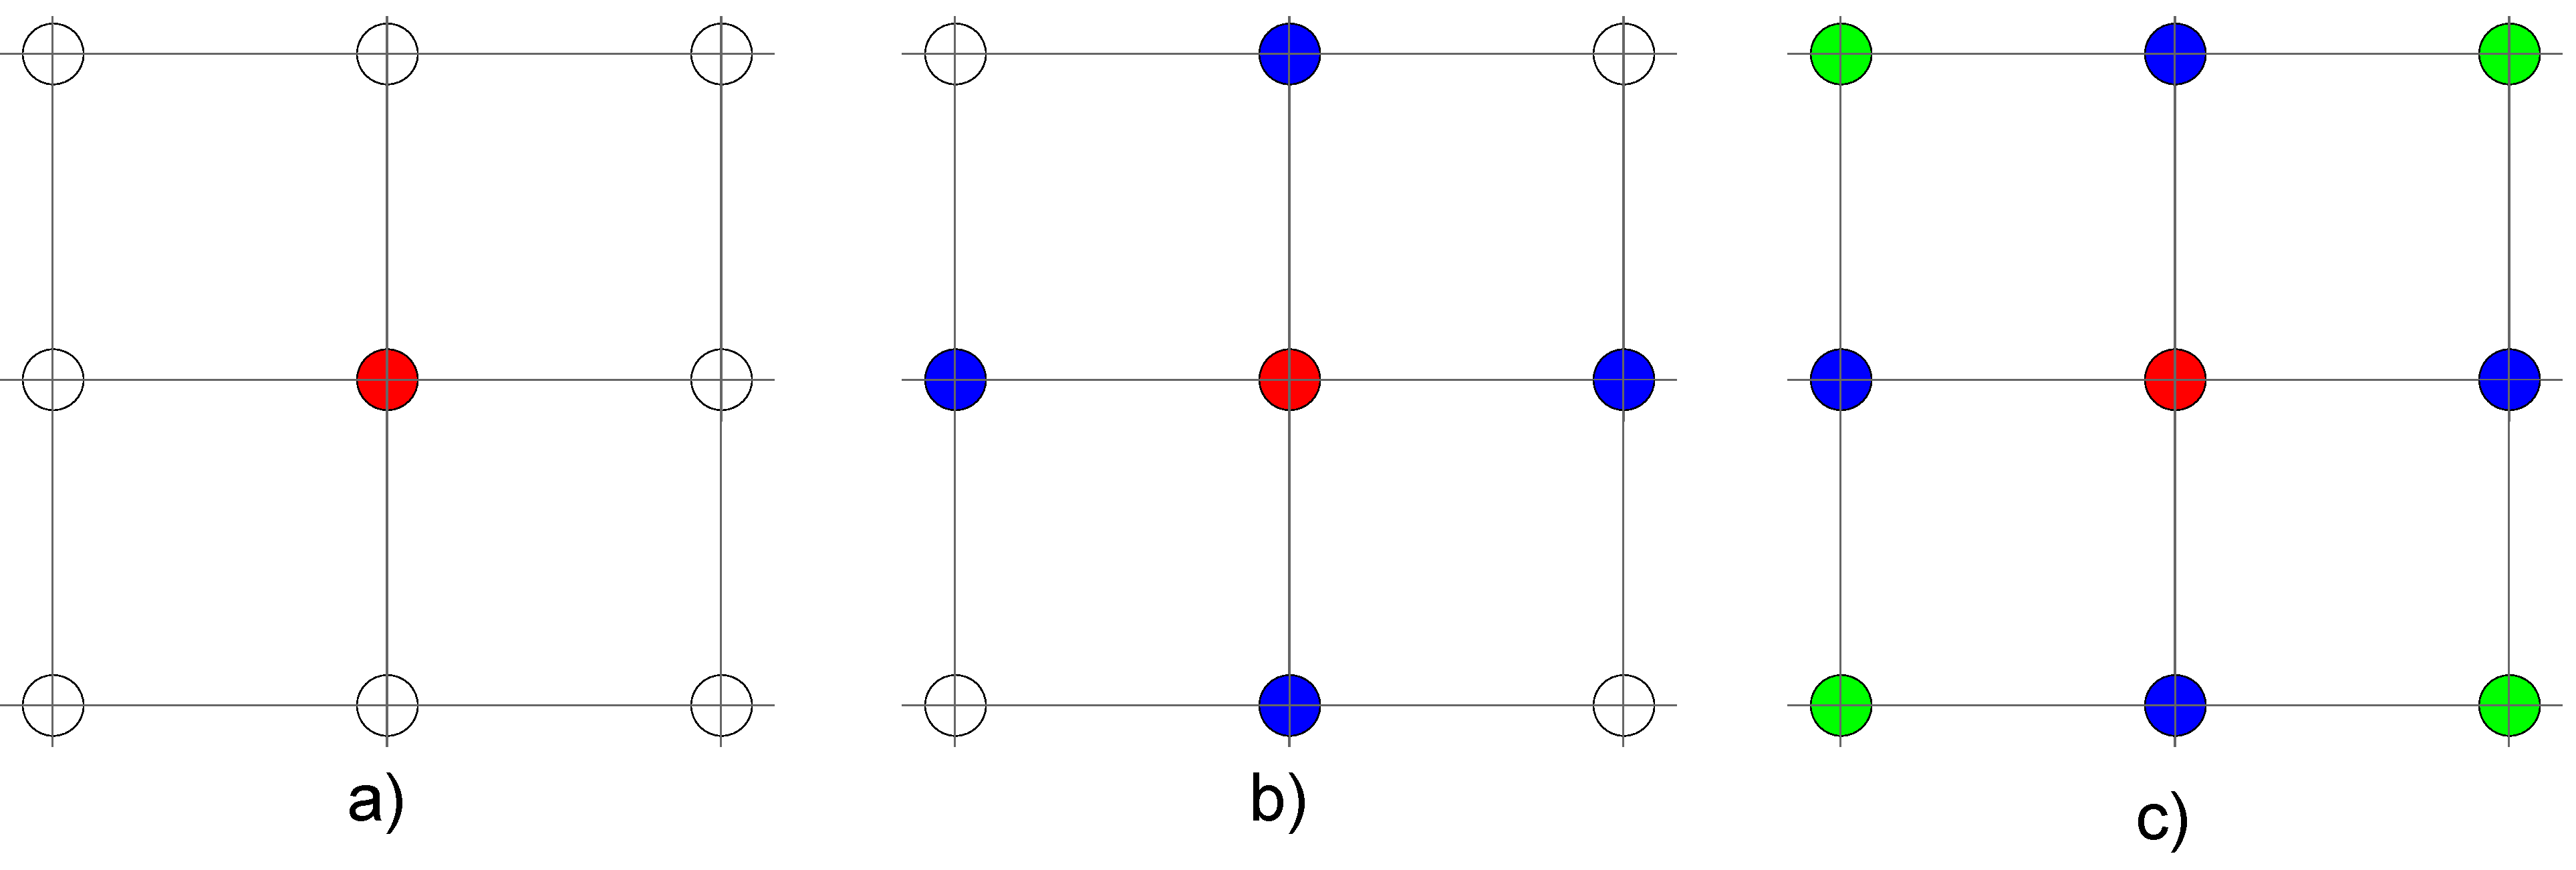
\includegraphics[width=0.8\textwidth]{chapters/chapter02/mg_restriction_operators}
	\caption{\textbf{a)} The injection operator just copies a point from a fine grid to a coarse grid. \textbf{b)} and \textbf{c)} The half weighting and full weighting operators calculate the average of five or nine points, respectively. }
	\label{fig:mg_restriktion_op}
\end{figure}

The \textbf{full weighting operator} applied to a grid function $d_h$ is

\begin{align}
d_{2h}(x,y) &= I_h^{2h} d_h(x,y)\nonumber \\
&=  \frac{1}{16}\begin{bmatrix}
1 & 2 & 1\\
2 & 4 & 2\\
1 & 2 & 1\\
\end{bmatrix}_h^{2h} d_h(x,y) \\
& = \frac{1}{16} \Big(4 d_h(x,y) + 2 d_h(x+h,y) + 2 d_h(x-h,y) + 2 d_h(x,y+h) + 2 d_h(x,y-h) \nonumber \\ 
& + d_h(x+h,y+h) + d_h(x-h,y-h) + d_h(x+h,y-h) + d_h(x-h,y+h)\Big ) \nonumber
\end{align}
and similarly, the \textbf{half weighting operator} applied to  a grid function $d_h$ can be written as
\begin{align}
d_{2h}(x,y) &= I_h^{2h} d_h(x,y)\nonumber \\
&=  \frac{1}{16}\begin{bmatrix}
0 & 1 & 0\\
1 & 4 & 1\\
0 & 1 & 0\\
\end{bmatrix}_h^{2h} d_h(x,y) \\
& = \frac{1}{8} \Big(4 d_h(x,y) +  d_h(x+h,y) +  d_h(x-h,y) +  d_h(x,y+h) +  d_h(x,y-h) \Big ) \nonumber 
\end{align}

All mentioned restriction operators can be seen in Fig.~\ref{fig:mg_restriktion_op}.

\subsection{Interpolation}
For the transition from a coarse grid $\Omega_{2h}$ to a finer grid $\Omega_h$ (Step 2d in the two-grid cycle) an interpolation is used. Fig.~\ref{fig:mg_prolongation_grid} shows a fine grid that was obtained after calculating missing points with the help of the coarse grid points (in red). For a two-dimensional grid, a bilinear interpolation is suitable. An example for that is illustrated in Fig.~\ref{fig:mg_prolongation}. In this example, the red points were already part of the coarse grid and are just copied to the corresponding points on the fine grid. The other points are determined by an averaging process:

\begin{align}
I_{2h}^h d_{2h}(x,y) =
  \begin{cases}
    d_{2h}(x,y)                                      & \quad \text{for red}\\
    \frac{1}{2} \big ( d_{2h}(x,y+h) + d_{2h}(x,y-h) & \quad \text{for yellow}\\
    \frac{1}{2} \big ( d_{2h}(x+h,y) + d_{2h}(x-h,y) & \quad \text{for blue}\\
    \frac{1}{2} \big ( d_{2h}(x+h,y+h) + d_{2h}(x-h,y+h) \\
    + \big ( d_{2h}(x+h,y-h) + d_{2h}(x-h,y-h) & \quad \text{for green}
  \end{cases}
\end{align}

The interpolation operator $I_2h^h$ can also be written in stencil notation, in a very similar way as the restriction operator for full weighing:

\begin{equation}
I_{2h}^h = \frac{1}{4} \begin{bmatrix}
1 & 2 & 1\\
2 & 4 & 2\\
1 & 2 & 1\\
\end{bmatrix}_{2h}^{h} 
\end{equation}

\begin{figure}[h]
	\centering
	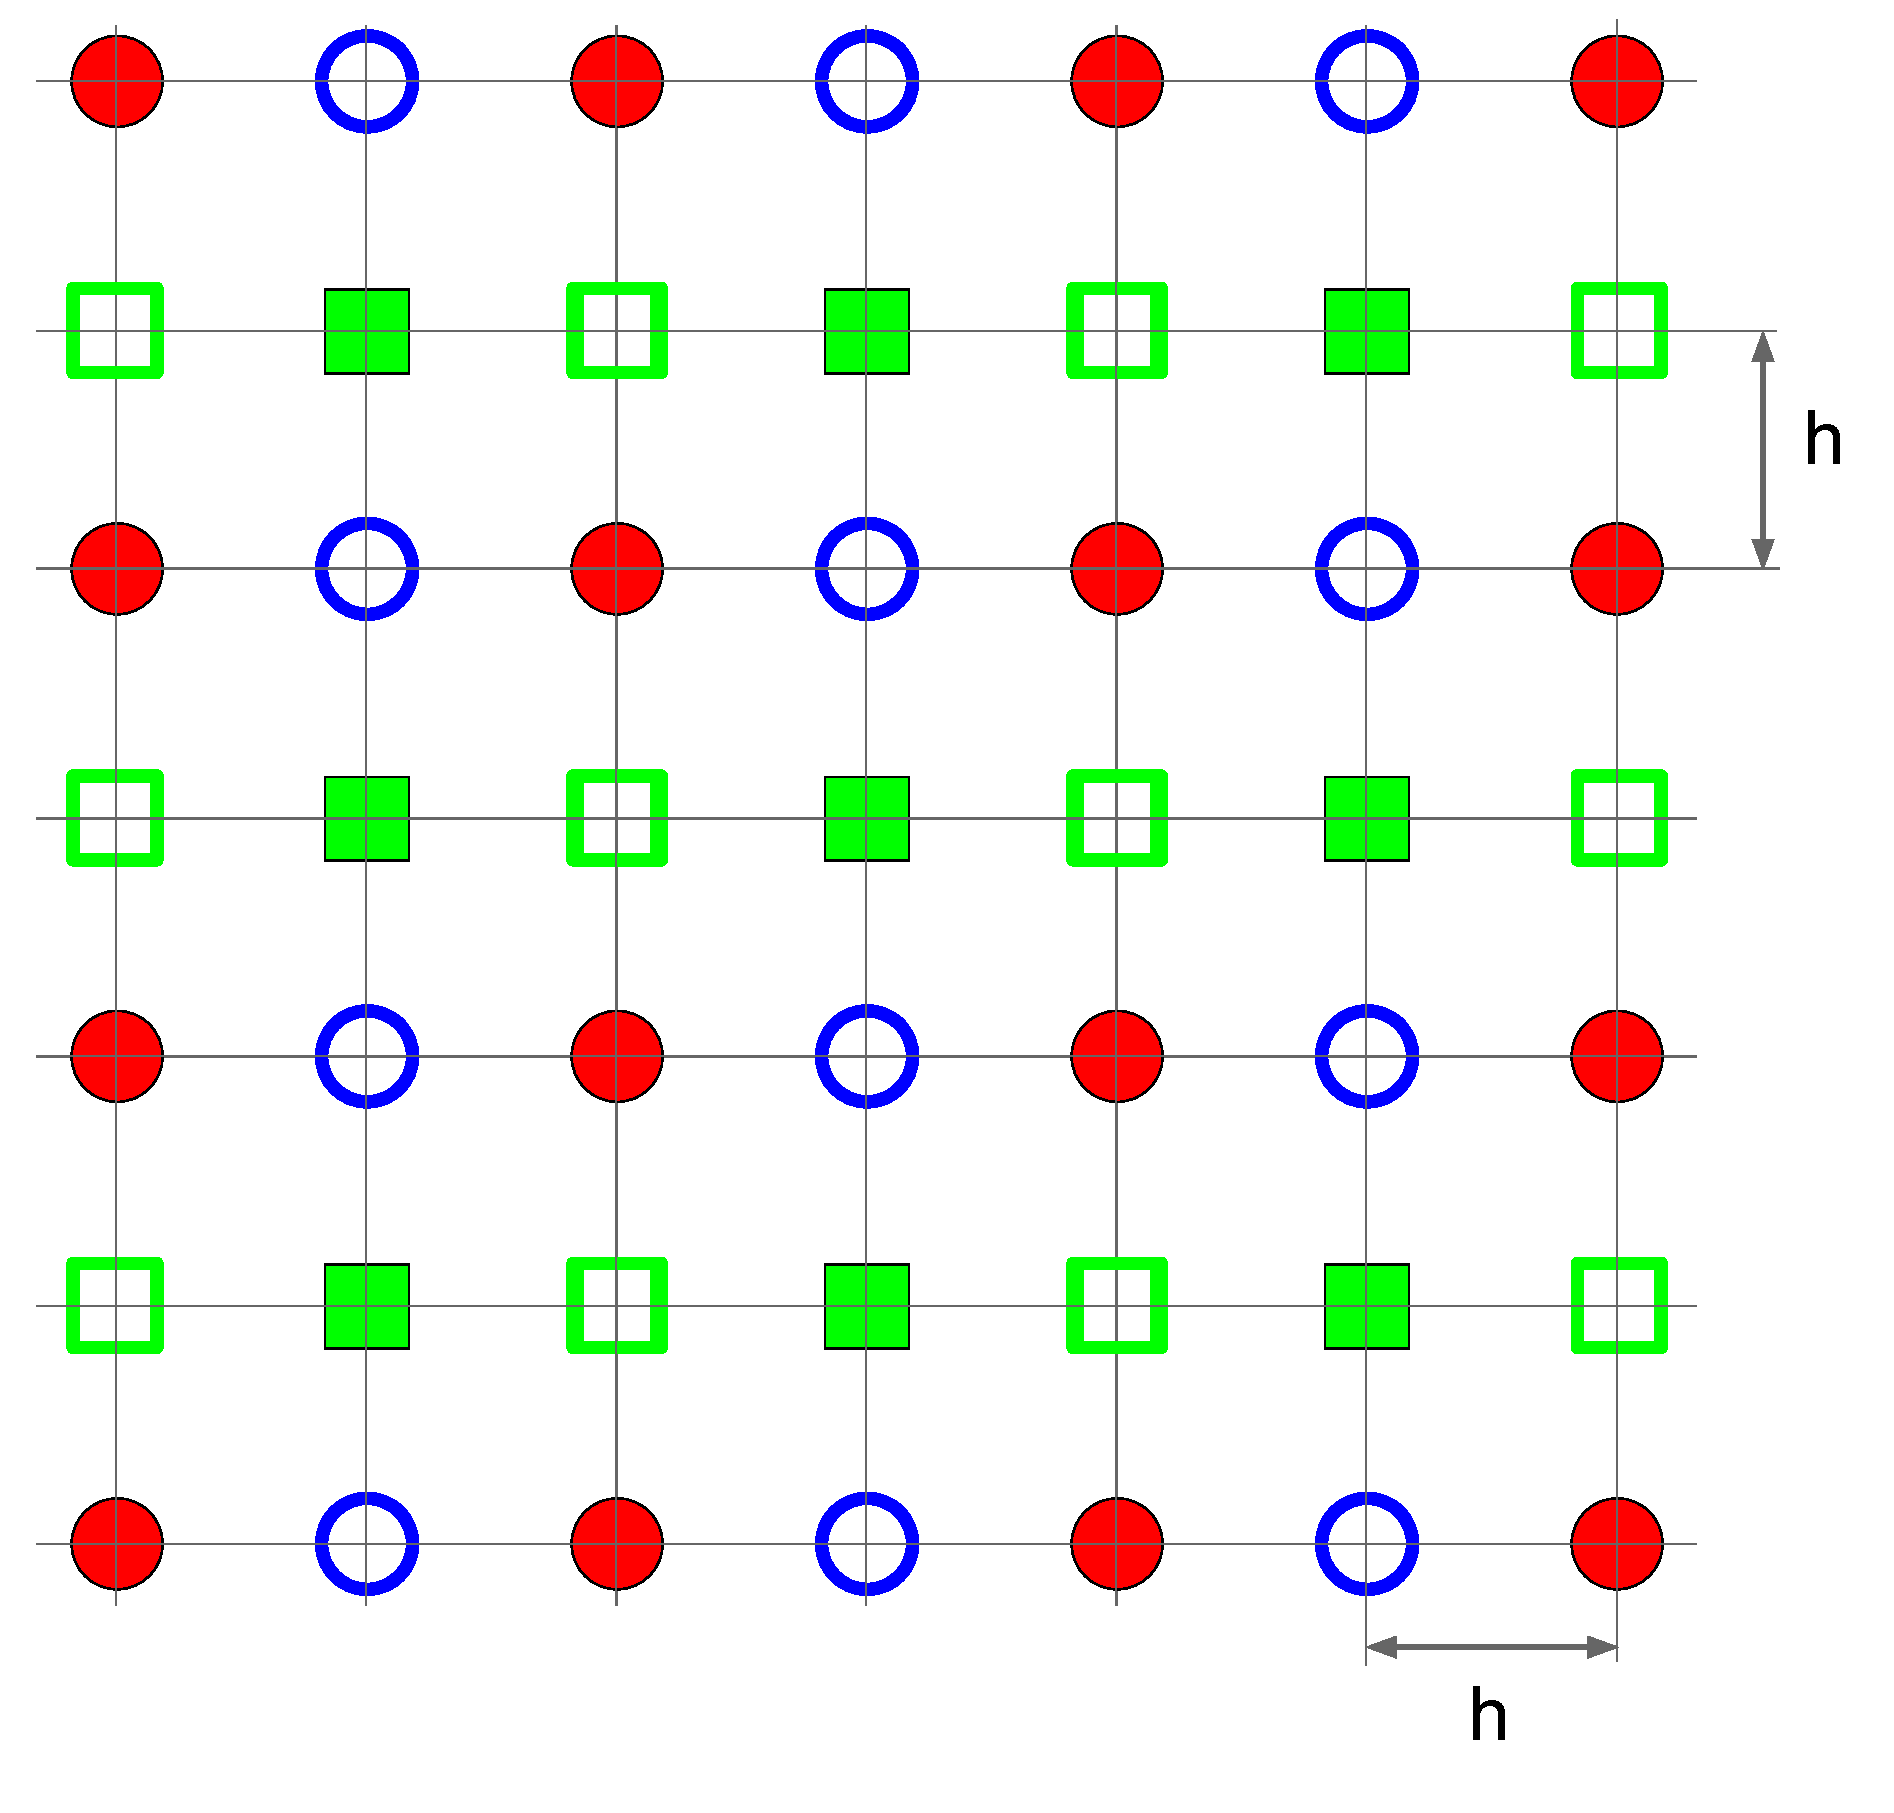
\includegraphics[width=0.5\textwidth]{chapters/chapter02/mg_prolongation_grid}
	\caption{Transitioning to a fine grid $\Omega_h$: The red points were already part of the rough grid $\Omega_H$, while the other points are calculated by interpolation.}
	\label{fig:mg_prolongation_grid}
\end{figure}

Fig.~\ref{fig:mg_prolongation} shows how the new grid points are calculated by averaging the red grid points.

\begin{figure}[h]
	\centering
	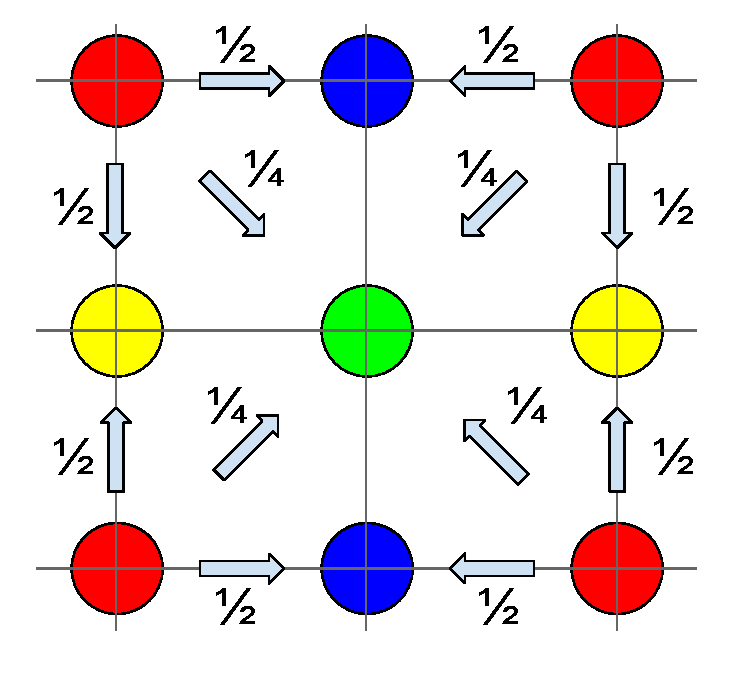
\includegraphics[width=0.5\textwidth]{chapters/chapter02/mg_prolongation}
	\caption{The fine grid values of new points are calculated by taking the average of values of the old grid.}
	\label{fig:mg_prolongation}
\end{figure}


\subsection{Coarse Grid Operator $L_H$}
In order to solve the system $L_H v_h^m = \overline{d}_H^m$ from the two-grid cycle on the coarser grid, first the coarse grid operator $L_H$ has to be determined. Even though it only has to be calculated once and not in each iteration step, this can take a considerable ratio of the total time spent on the multigrid iteration. The coarse grid operator can be determined by either discretizing the grid again, or by performing the matrix multiplication
\begin{equation}
L_H = I_h^H L_h I_H^h
\end{equation}
with the restriction and interpolation operators $I_h^H$ and $I_H^h$. When solving big problems of the Poisson equation, the matrices of this equation are all very big and very sparse, so efficient algorithms are needed. In fact, this multiplication was the part of the thesis where most practical work had to be done and existing algorithms were to be improved. These matrix multiplications will be extensively discussed in the next chapter. 

\subsection{Other Components}
The steps 2a), 2c) and 2e) of the two-grid cycle have not been described yet. For 2a) the computation of the defect on the fine grid, there is just a matrix-vector multiplication and a  vector subtraction. Step 2c), solving the defect equation for the error on the coarse grid, uses an iterative or direct solver. This  can, but does not have to be the relaxation method used for Step 1 and Step 3. Step 2e), computing a new approximation, is just a vector addition. 

\section{Multigrid Cycle}
\label{sec:multigrid_cycle}
The two-grid cycle that was discussed earlier has much better convergence properties than iterative solvers on their own. However, the convergence properties can still be further improved: In the two-grid cycle, the error $v_h^m$ is computed through solving the system $L_H v_H^m = d_H^m$. Since the iterative method for solving this system is again very suitable for smoothing, but not so much for making the error small, another coarse grid correction can be applied to the coarser grid instead of solving the coarse grid defect equation exactly.  The smoothing and coarse grid correction methods can be performed so often, that $L_H v_H^m = d_H$ is always applied to a grid of a certain size, e.g. a grid $\Omega_{\frac{1}{4}}$. That way, errors of errors are calculated and added to an error, until the finest error is added to the solution $u_h$. 

Fig.~\ref{fig:mg_cycles} shows different multigrid cycles (one iteration each) for different numbers of grids and different cycle indices $\gamma$. The cycle index $\gamma$ tells how many two-grid iteration steps are performed. The cycles with $\gamma = 1$ are called V-cycles and the cycles with $\gamma = 2$ are called W-cycles.

\begin{figure}[tbp]
	\centering
	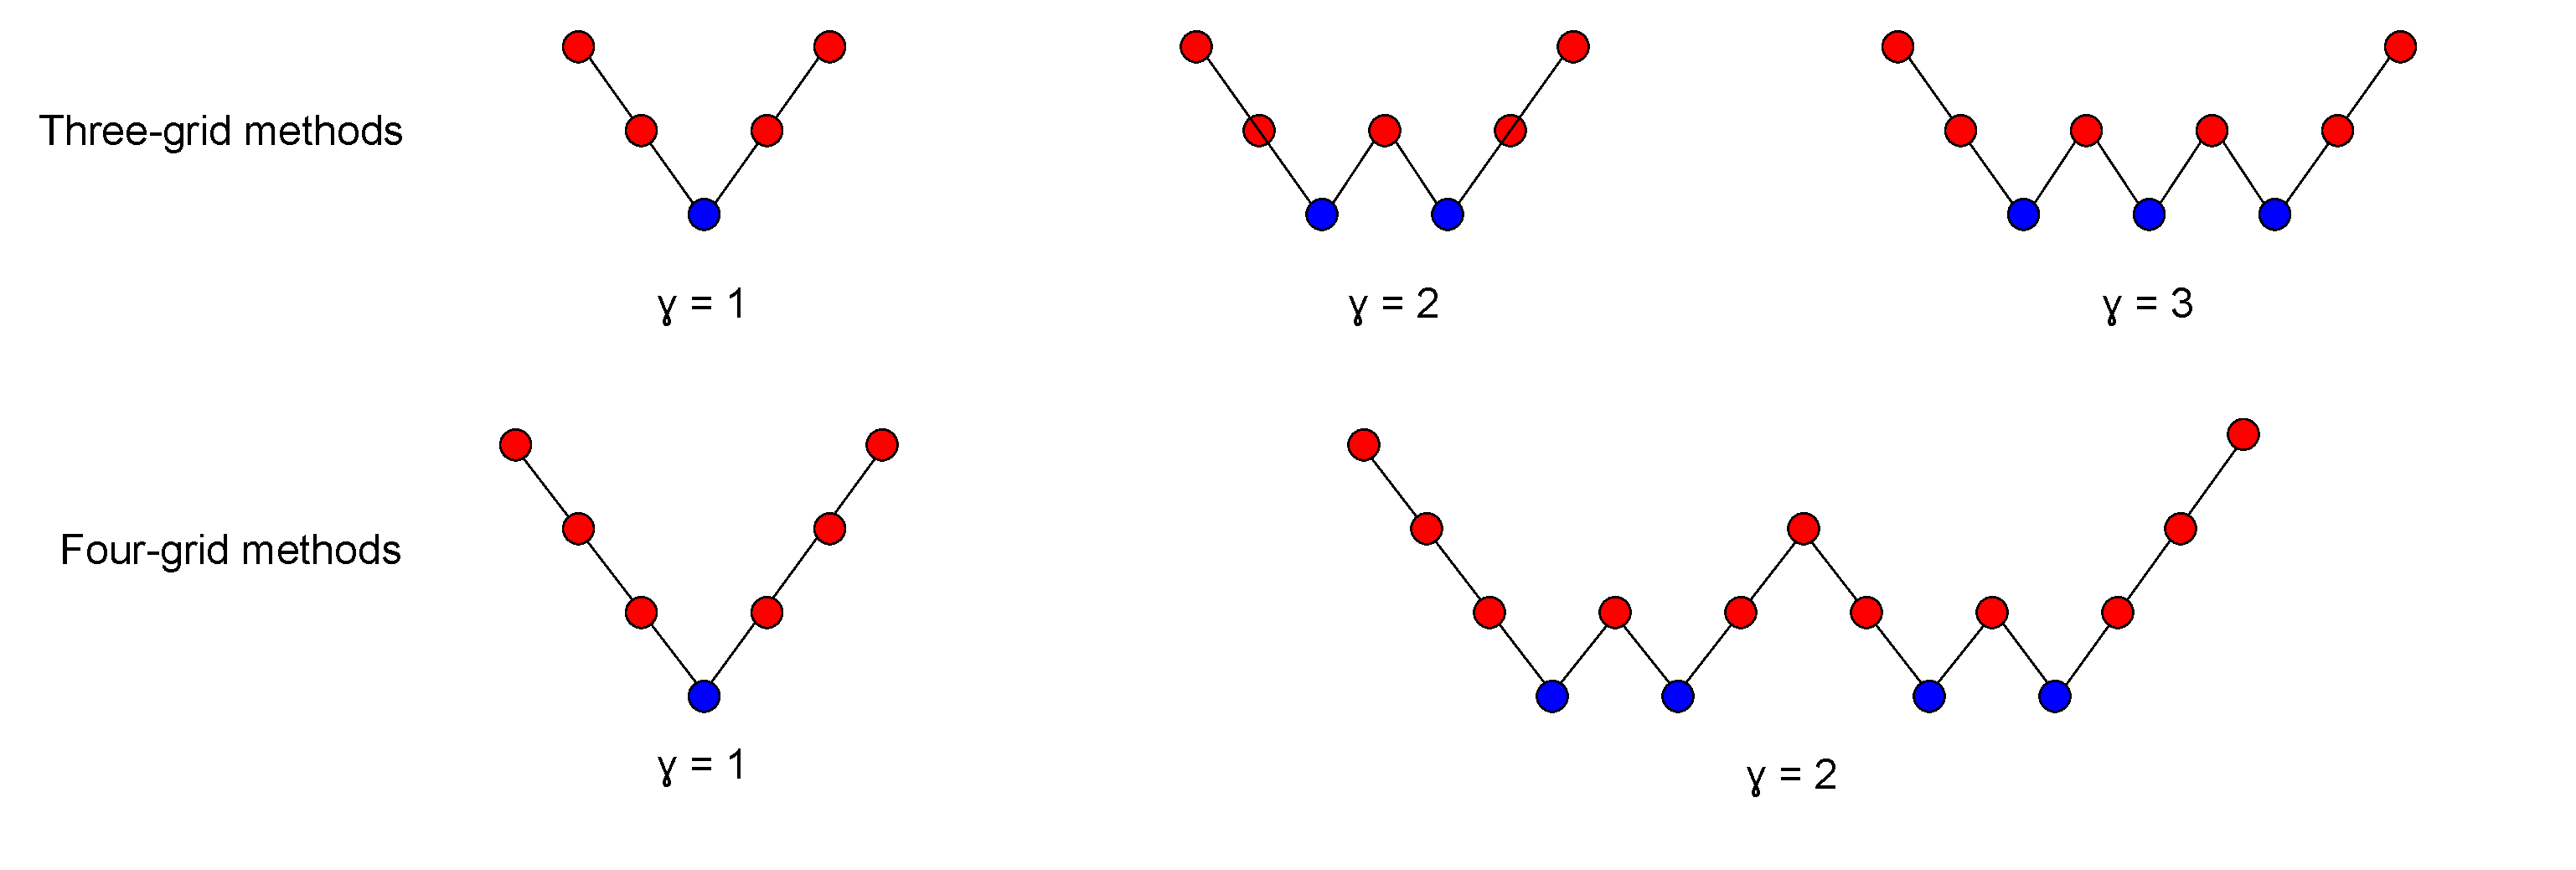
\includegraphics[width=1.07\textwidth]{chapters/chapter02/mg_cylces}
	\caption{Different multigrid cycles four three- and four-grid methods and for different $\gamma$. On the coarsest grid, an exact solution is computed (in blue), while on all other grids smoothing is applied (red).}
	\label{fig:mg_cycles}
\end{figure}

Of course there are also many other possibilities to run a multigrid cycle, also with non-constant $\gamma$ and non-constant numbers of presmoothing and postsmoothing steps $\nu_1$ and $\nu_2$.


A multigrid cycle (a multigrid iteration) can be seen as a function that takes the following as input (the index $l$ stands for the current grid level and the first level is  the finest one: $l = k$): 
\begin{itemize}
\item the current grid level $l$ (out of $k$ levels in total),
\item the cycle index $\gamma$
\item an approximation $u_l^{m}$, 
\item a linear operator $L_l$,
\item the function $f_l$, and 
\item the number of presmoothing and postsmoothing steps, $\nu_1, \nu_2$. 
\end{itemize}
The output is a new approximation $u_k^{m+1}$:
Like the two-grid cycle, the multigrid cycle also comprises three basic steps and runs like shown in Algorithm 2. 
\vspace{5mm}

\begin{algorithm}[h]
\fbox{%
\begin{minipage}{0.94\textwidth}
\textbf{Multigrid Cycle:} \hspace{15mm} $u_k^{m+1} = \textbf{MGCycle}(k, \gamma, u_k^m, L_k, f_k, \nu_1, \nu_2)$
\begin{enumerate}
\item \textbf{Presmoothing:} A relaxation method (e.g. Gauss-Seidel or Jacobi) is applied $\nu_1 \geq 0$ times to smoothen $u_h^m$ and obtain a smooth $\overline{u}_h^m$.
\item \textbf{Coarse grid correction:} 
\begin{enumerate}
\item Compute the defect: $\hspace{55mm}\overline{d}_k^m = f_k - L_k \overline{u}_k^m$
\item Transfer the defect to a coarser grid:  $\hspace{25mm} \overline{d}_{k-1}^k = I_k^{k-1} \overline{d}_k^m$
\item Compute an approximate solution of the defect equation $v_{k-1}^m$: 

\center $ L_{k-1} v_{k-1}^m = \overline{d}_{k-1}^m$
\begin{itemize}
\item If $k = 1$, use a direct or iterative solver and solve it exactly.
\item If $k>1$, call the multigrid function recursively, with $\gamma$ iterations and a zero vector as an initial approximation:
\center $v_{k-1}^m$ = MG\_Cycle($k-1, \gamma, 0, L_{k-1}, \overline{d}_{k-1}^k, \nu_1, \nu_2) $
\end{itemize}
\item Transfer the error to a finer grid: $\hspace{25mm} v_k^m = I_{k-1}^k v_{k-1}^m$
\item Compute a new approximation: $\hspace{29mm}   u_k^{new} = \overline{u}_k^m + v_k^m$
\end{enumerate}
\item \textbf{Postsmoothing:} The new approximation $u_k^{m+1}$ is obtained through smoothing $u_k^{new}$ for $\nu_2 \geq 0$ times.
\end{enumerate}
\vspace{1mm}
\end{minipage}}
\vspace{5mm}
\label{alg:multigrid_cycle}
\caption{Multigrid cycle}
\end{algorithm}

The main difference to the two-grid cycle is Step 2c) in the algorithms (solving the defect equation): For the two-grid cycle it is solved exactly, while the multicycle iteration uses an approximate solution that is obtained by an recursive call of the multicycle function. Only on the coarsest grid the multicycle iteration performs an exact calculation. 



\section{Parallelizing Multigrid}
In order to get a high performance performance, it is necessary to parallelize the multigrid method. The degree of parallelism depends on the different components of multigrid (error smoothing, restriction, ...). 

As mentioned earlier, the relaxation methods offer different degrees of parallelization: The Jacobi method is always fully parallelizable, while the lexicographical Gauss-Seidel method  has a can only run on up to $\sqrt{\#\Omega_h}$ processes at the same time and the red-black Gauss-Seidel iteration on $\frac{1}{2} \#\Omega_h$ processes. The idea of red-black ordering can also be generalized to multi-colour relaxations, which are also highly parallel \cite{Trottenberg:2000:MUL:374106}.

In order to fully exploit the degree of parallelism of a fully parallel relaxation method (e.g. Jacobi smoothers), the hardware on which the problem is computed has as many computing cores as there are points in the grid\footnote{This is neither a realistic scenario for a fine grid, nor is this desirable due to network latencies.}. However, when the computation continues and reaches very coarse grids, the work cannot be split in a reasonable way to a high number of processors, so many processors stay idle for some time. The same thing can be said about the restriction and interpolation methods, so in some stages of the cycle the algorithm can be much more parallelized than in other stages.

A stage of multigrid that can be very computationally intensive is the sparse matrix-matrix multiplication that is needed for the computation of linear operators $L_H$. This is also a step whose size depends on the current grid level and it can be  parallelized very well. In the next chapter, this matrix multiplication is illustrated in much detail.



%=========================================================